\documentclass{article}
\usepackage{amsmath}
\usepackage[utf8]{inputenc}
\usepackage{float}
\usepackage{epsfig,graphicx}
\usepackage{xcolor,import}
\usepackage[german]{babel}
\usepackage{textcomp}
\usepackage{mathtools}

\begin{document}
\thispagestyle{empty}
			\begin{center}
			\Large{Fakultät für Physik}\\
			\end{center}
\begin{verbatim}


\end{verbatim}
							%Eintrag des Wintersemesters
			\begin{center}
			\textbf{\LARGE WINTERSEMESTER 2014/15}
			\end{center}
\begin{verbatim}


\end{verbatim}
			\begin{center}
			\textbf{\LARGE{Physikalisches Praktikum 1}}
			\end{center}
\begin{verbatim}




\end{verbatim}

			\begin{center}
			\textbf{\LARGE{PROTOKOLL}}
			\end{center}
			
\begin{verbatim}





\end{verbatim}

			\begin{flushleft}
			\textbf{\Large{Experiment Nr.9:} Gleichstrom}\\
							%Experiment Nr. und Titel statt den Punkten eintragen
			\LARGE{}	
			\end{flushleft}

\begin{verbatim}

\end{verbatim}	
							%Eintragen des Abgabedatums, oder des Erstelldatums des Protokolls
			\begin{flushleft}
			\textbf{\Large{Datum:}} \Large{12.12.2014}
			\end{flushleft}
			
\begin{verbatim}
\end{verbatim}
							%Namen der Protokollschreiber
		\begin{flushleft}
			\textbf{\Large{Namen:}} \Large{Veronika Bachleitner, Erik Grafendorfer}
			\end{flushleft}

\begin{verbatim}


\end{verbatim}
							%Kurstag und Gruppennummer, zb. Fr/5
			\begin{flushleft}
			\textbf{\Large{Kurstag/Gruppe:}} \Large{Fr/1}
			\end{flushleft}

\begin{verbatim}






\end{verbatim}
							%Name des Betreuers, das Praktikum betreute.
			\begin{flushleft}
			\LARGE{\textbf{Betreuer:}}	\Large{}	
			\end{flushleft}
\newpage	

\section{Photovoltaische Solarzellen als Gleichstromquelle}

\subsection{Aufgabenstellung}
\subsection{Grundlagen}
\subsection{Versuchsaufbau und Methoden}
\subsection{Durchführung}
\subsection{Ergebnisse}
RL 1kOhm +- 5%, +- 0.25% Lin
RI 0.517 Ohm

\subsection{Diskussion}

\section{Widerstandsbestimmung mittels Wheatstone Brücke}

\subsection{Aufgabenstellung}
Wir messen drei unbekannte Widerstände mit Hilfe einer Brückenschaltung.
Außerdem messen wir den Gesamtwiderstand zweier Widerstände einmal in einer Reihenschaltung und einmal in einer Parallelschaltung und vergleichen unsere Messungen mit berechneten Ergebnissen.
\subsection{Grundlagen}
\subsection{Versuchsaufbau und Methoden}
\subsection{Durchführung}
\subsection{Ergebnisse}
Testwiderstand R0: 1kOhm
\subsection{Diskussion}

\section{Reale Spannungsquelle}

\subsection{Aufgabenstellung}
\subsection{Grundlagen}
\subsection{Versuchsaufbau und Methoden}
\subsection{Durchführung}
\subsection{Ergebnisse}
Leerlaufspannung:
1.505V

Messwerte:
\begin{tabular}{r|l}
\hline
U [V] & I [mA]\\
\hline
1.494 & 7.43\\
1.494 & 8.26\\
1.492 & 9.27\\
1.491 & 10.59\\
1.489 & 12.32\\
1.487 & 14.73\\
1.483 & 18.33\\
1.477 & 24.27\\
1.466 & 35.94\\
1.445 & 69.2\\
\hline
\end{tabular}

a  = -0.000995923244695565 +/- 1.3967318979964e-05
b  = 1.50150717852848 +/- 0.000251022348272116
--------------------------------------------------------------------------------------
Chi2/doF = 1.35308792311826e-07
R2 = 0.998625088078122

Leerlaufspannung hat sich um 0.001 V verringert

Fluke 183:
5V DC
~mA

\subsection{Diskussion}

\section{Belasteter Spannungsteiler}

\subsection{Aufgabenstellung}
Wir bestimmen aus einer einfachen Schaltung, dem Spannungsteiler, die elektrischen Widerstände von drei Lastwiderständen mit zwei Spannungsmessgeräten.
\subsection{Grundlagen}
Wenn ein Potentiometer seinen Gesamtwiderstand R aufteilt in $R_1$ und (R-$R_1$), erhält man mittels der Kirchhoffschen Regeln für einen Lastwiderstand $R_L$ der zu $R_1$ parallel geschalten ist folgende Beziehung: 
\begin{equation}
\label{spannungsteiler}
\frac{U_L}{U}=\frac{R_1R_L}{R_LR+R_1(R-R_1)}
\end{equation}
$U_L$ bezeichnet die Klemmenspannung am Lastwiderstand $R_L$, U die Gesamtspannung. Wir führen weitere Bezeichnungen ein:
\begin{align*}
r_L=\frac{R_L}{R} \\
r_1=\frac{R_1}{R} \\
u = \frac{U_L}{U}
\end{align*}
Mit diesen erhalten wir schließlich für den Lastwiderstand $R_L$:
\begin{equation*}
r_L=-\frac{u\cdot r_1(1-r_1)}{u-r_1}
\end{equation*}
\begin{equation}
\label{spannungsteiler_umgeformt}
R_L=-R\cdot \frac{u\cdot r_1(1-r_1)}{u-r_1}
\end{equation}

\subsection{Versuchsaufbau und Methoden}
Wir schalten einen Lastwiderstand parallel zu einem Teilwiderstand eines Potentiometer und in Serie zu seinem anderen Teilwiderstand und messen mit zwei gleichen Spannungsmessgeräten die Spannungen am Teilwiderstand und an allen Widerständen. Mit (\ref{spannungsteiler}) und dem Verhältnis der Teilwiderstände am Potentiometer ermitteln wir dann den Lastwiderstand. 
\subsection{Durchführung}
Wir verwenden zwei Fluke 183 Multimeter, die im Bereich von 5V Gleichspannung mit 5000 Zählimpulsen zu 1 mV auf $\pm (0.07\%$ +1 Zählimpuls) genau messen.
\subsection{Ergebnisse}
\begin{center}
\begin{figure}
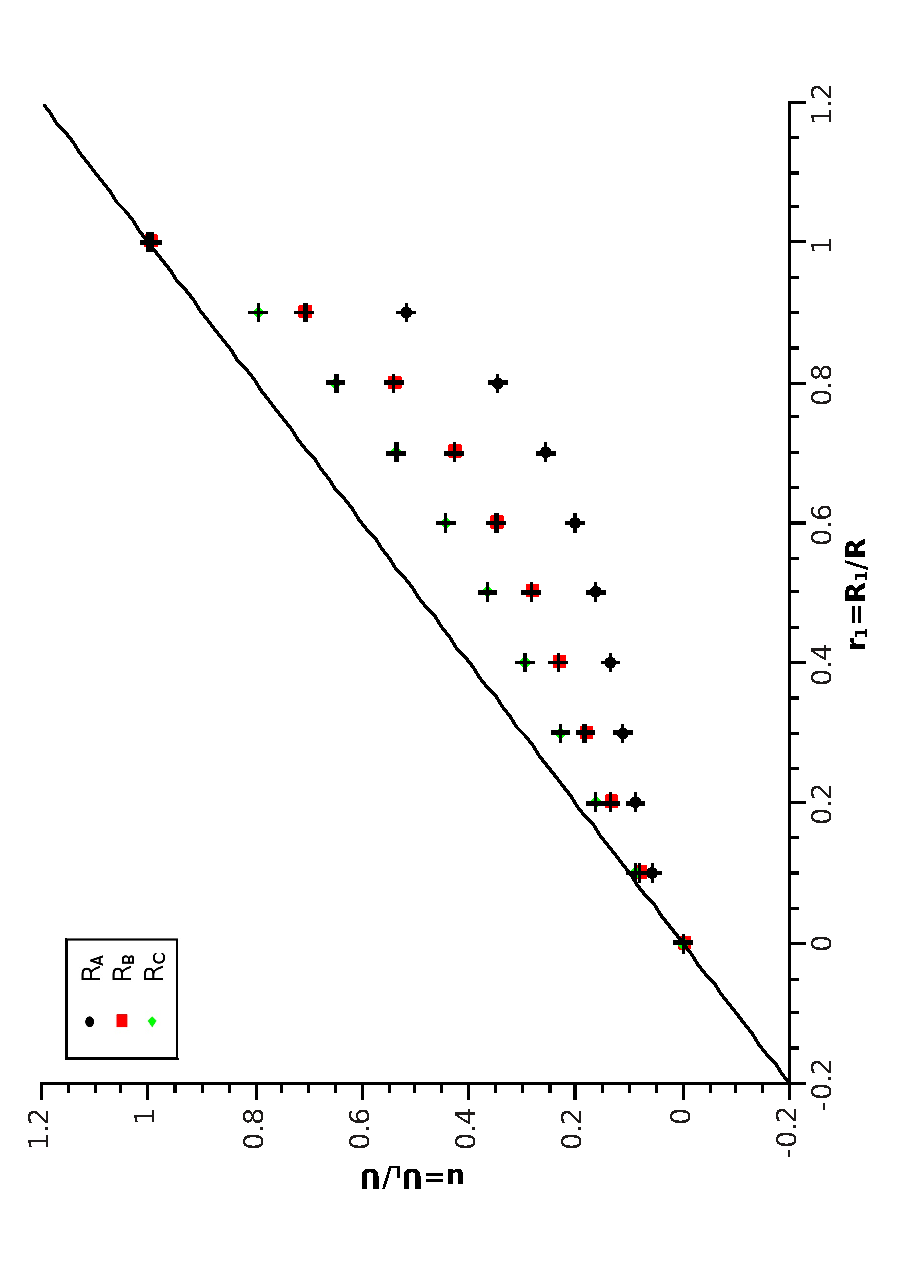
\includegraphics[scale=0.5,angle=-90]{spannungsteiler.eps}
\end{figure}
\end{center}
Mit  (\ref{spannungsteiler_umgeformt}) und Größtfehlerabschätzung:

$$R_A=(1221\pm6) \Omega$$
$$R_B=(3321 \pm 11) \Omega $$
$$R_C=(6831 \pm 31) \Omega $$

\subsection{Diskussion}
\end{document}
